%!TEX root = ../main.tex

%======================================
% 1. Einleitung
%======================================
\input{content/01_Einleitung.tex}

%======================================
% 2. Theoretische Grundlagen
%======================================
%!TEX root = ../main.tex

\chapter{Theoretische Grundlagen}
\label{chap:theoretische_grundlagen}

Für das Verständnis der in dieser Arbeit behandelten Prüfzifferverfahren sind einige grundlegende mathematische Konzepte und Definitionen notwendig. Diese Grundlagen sollen im Folgenden kurz erläutert werden.



\section{Fehlererkennung vs. Fehlerkorrektur}

Bei der Informationsübertragung und -speicherung unterscheidet man grundsätzlich zwei Arten des Umgangs mit Fehlern:

\begin{itemize}
    \item \textbf{Fehlererkennung:} Ein Verfahren zur Fehlererkennung ermöglicht die Detektion von Übertragungsfehlern mittels redundanter Information, kann jedoch die ursprüngliche Nachricht nicht rekonstruieren. Prüfzifferverfahren implementieren in der Regel ausschließlich diese Funktionalität.

    \item \textbf{Fehlerkorrektur:} Diese fortgeschritteneren Verfahren ermöglichen nicht nur die Erkennung, sondern auch die Korrektur von Fehlern ohne erneute Übertragung der Originaldaten. Sie basieren auf komplexeren mathematischen Konstrukten wie Hamming-Codes oder Reed-Solomon-Codes und erfordern einen höheren Grad an Redundanz.
\end{itemize}



\section{Galoiskörper} \label{sec:galois_fields}
Galoiskörper, benannt nach dem französischen Mathematiker Évariste Galois, sind endliche Körper basierend auf den Restklassen \(\mathbb{Z}_p\). Sie zeichnen sich dadurch aus, dass sie eine endliche Anzahl von Elementen besitzen und alle Körperaxiome erfüllen, wie etwa die Existenz von neutralen Elementen für Addition und Multiplikation sowie die Invertierbarkeit der Elemente bezüglich dieser Operationen \cite{Springer_RS}.

Es existieren die Galoiskörper \(GF(p^n)\), deren Anzahl an Elementen immer eine Potenz einer Primzahl ist, wobei \(p\) die Primzahl und \(n\) eine positive ganze Zahl ist. Es gibt beispielsweise einen Körper mit \(2^3 = 8\) Elementen, aber keinen mit \(10\) Elementen. Für \(n = 1\) entspricht der Galoiskörper \(GF(p^1)\) dem bekannten Restklassenkörper \(\mathbb{Z}_p\), der aus den Restklassen modulo \(p\) besteht \cite{Springer_RS}.

Die Konstruktion von Galoiskörpern für \(n > 1\) erfolgt durch die Erweiterung von \(\mathbb{Z}_p\) mittels irreduzibler Polynome. Ein irreduzibles Polynom über \(\mathbb{Z}_p\) ist ein Polynom, das sich nicht in Faktoren zerlegen lässt, die ebenfalls in \(\mathbb{Z}_p\) liegen. Die Elemente des Galoiskörpers \(GF(p^n)\) sind dann die Restklassen von Polynomen modulo eines solchen irreduziblen Polynoms mit dem Grad \(n\). Soll beispielsweise der Galoiskörper \(GF(2^3)\) konstruiert werden, so wird ein solches irreduzibles Polynom \(g(x)= x^3 + x + 1\) mit dem Grad \(n = 3\) über \(\mathbb{Z}_2\) benötigt. Die Elemente des Körpers sind dann die Restklassen der Polynome modulo \(g(x)\), haben entsprechend einen maximalen Grad von \(n - 1 = 2\), eine Form von \(a_1 x^2 + a_2 x^1 + a_3 x^0\) und die möglichen Koeffizienten sind die Elemente von $\mathbb{Z}_2$: \(0\) oder \(1\) \cite{Springer_RS}. Es ergeben sich die folgenden Elemente, welche sich auch als Binärzahlen interpretieren lassen (vgl. Tabelle~\ref{tab:gf8}):

\begin{table}[H]
    \centering
    \begin{tabular}{|c|c|}
        \hline
        Element & Binärdarstellung \\
        \hline
        \(0\) & \(000\) \\
        \(1\) & \(001\) \\
        \(x\) & \(010\) \\
        \(x + 1\) & \(011\) \\
        \(x^2\) & \(100\) \\
        \(x^2 + 1\) & \(101\) \\
        \(x^2 + x\) & \(110\) \\
        \(x^2 + x + 1\) & \(111\) \\
        \hline
    \end{tabular}
    \caption{Elemente des Galoiskörpers \(GF(2^3)\)}
    \label{tab:gf8}
\end{table}

Die Addition in Galoiskörpern erfolgt komponentenweise (in $\mathbb{Z}_2$ per XOR), während die Multiplikation durch die Division des Produkts zweier Polynome (die beiden Elemente) mit dem irreduziblen Polynom \(g(x)\) und der Verwendung des Restes als Ergebnis definiert ist. Für größere Körper wird die Multiplikation häufig durch die Verwendung einer primitiven Einheitswurzel \(\alpha\) vereinfacht, die als Generator für die Elemente des Körpers dient \cite{Springer_RS}.

Galoiskörper sind besonders nützlich in der Praxis, da sie effiziente Berechnungen ermöglichen. Insbesondere die Körper \(GF(2^n)\) sind aufgrund ihrer einfachen Implementierung in Hardware weit verbreitet. Sie finden Anwendung in Reed-Solomon-Codes, die beispielsweise in DVDs und anderen digitalen Speichermedien zur Fehlerkorrektur eingesetzt werden \cite{Springer_RS}.


%======================================
% 3. Klassifikation von Prüfzifferverfahren mit Detailbeispielen
%======================================
% %!TEX root = ../../main.tex

\chapter{Klassifikation der Prüfzifferverfahren}
\label{ch:klassifikation}

Die Welt der Prüfzifferverfahren ist vielfältig und facettenreich. Um einen strukturierten Überblick zu ermöglichen, werden diese Verfahren nach ihren mathematischen Grundprinzipien klassifiziert. Diese Klassifikation erleichtert nicht nur das Verständnis der Verfahren, sondern ermöglicht auch eine gezielte Auswahl je nach Anwendungsfall und Anforderungsprofil.

Im Folgenden werden vier Hauptkategorien von Prüfzifferverfahren vorgestellt, die sich in ihren mathematischen Grundlagen, ihrer Komplexität und ihren Fehlererkennungseigenschaften unterscheiden. Einfache Modulo-Verfahren nutzen die elementare Restklassenarithmetik für die Fehlererkennung. Sie sind leicht zu implementieren und zu verstehen, weshalb sie besonders in einfachen Anwendungsfällen zum Einsatz kommen, wie etwa bei älteren Bankleitzahlen Gewichtsverfahren erweitern das Konzept durch positionsabhängige Gewichtungsfaktoren und erhöhen dadurch die Fehlererkennungsleistung deutlich. Sie finden Anwendung in wichtigen Identifikationssystemen wie der ISBN für Bücher oder den EAN-Codes im Einzelhandel. Verfahren mit Permutation führen zusätzlich eine systematische Umordnung der Ziffern durch, wodurch komplexere Fehlertypen erkannt werden können. Der Luhn-Algorithmus für Kreditkartennummern ist hierfür ein Paradebeispiel. Polynomielle Verfahren schließlich repräsentieren die mathematisch anspruchsvollste Kategorie, basierend auf der Arithmetik von Polynomen über endlichen Körpern. Der CRC (Cyclic Redundancy Check) ist der wichtigste Vertreter dieser Kategorie und wird häufig in der digitalen Datenübertragung eingesetzt.

Für jede dieser Kategorien werden in den folgenden Abschnitten die mathematischen Grundlagen erläutert und anhand von konkreten Beispielen veranschaulicht. Dabei wird sowohl auf die theoretischen Aspekte als auch auf die praktische Anwendung eingegangen, um ein umfassendes Verständnis zu vermitteln \cite{Hoffmann2023-sv}.


% 3.1 Gewichtsverfahren mit Detailbeispielen
%!TEX root = ../../main.tex

\chapter{Gewichtsverfahren}
\label{chap:Gewichtsverfahren}

\section{EAN-13}
\label{sec:ean13}

Ein klassisches Beispiel für ein Gewichtsverfahren ist die Berechnung der Prüfziffer der \ac{EAN}, die insbesondere zur eindeutigen Identifikation von Handelsprodukten dient. Die EAN findet sich in der Regel sowohl im Klartext als auch in Form eines Strichcodes auf Produktverpackungen und Etiketten.

Die gebräuchliche EAN-13 besteht aus insgesamt 13 Ziffern, wobei die letzte Ziffer eine Prüfziffer darstellt. Diese wird mittels eines Modulo-10-Verfahrens ermittelt, um Eingabefehler (z. B. Zahlendreher oder Einzelfehler) zuverlässig zu erkennen.

Zur Berechnung der Prüfziffer werden die ersten 12 Ziffern positionsabhängig mit alternierenden Gewichten von 1 und 3 multipliziert. Anschließend werden die Produkte aufsummiert. Die Prüfziffer ergibt sich als diejenige Zahl, die zur gebildeten Summe addiert werden muss, um ein durch 10 teilbares Ergebnis zu erhalten. Formal ausgedrückt entspricht die Prüfziffer dem Wert, der notwendig ist, um die alternierend gewichtete Quersumme modulo 10 auf null zu ergänzen.

Die EAN-13 ist wie folgt aufgebaut:\newline
% EAN-13 Prüfzifferberechnung
\begin{equation}
v_0 v_1 v_2 v_3 v_4 v_5 v_6 v_7 v_8 v_9 v_{10} v_{11} v_{12}
\end{equation}

Für eine EAN-13 ist die Berechnung der Prüfziffer \( v_{12} \) wie folgt: \newline
\begin{equation}
\sum_{i \text{ gerade}} v_i + \sum_{i \text{ ungerade}} 3v_i \equiv 0 \pmod{10}
\end{equation}
Dieses Verfahren gewährleistet eine effiziente Plausibilitätskontrolle der EAN-Nummer im praktischen Einsatz \cite{Hoffmann2023-sv}.

\begin{figure}[H]
    \centering
    \begin{subfigure}{0.48\textwidth}
        \centering
        
\includegraphics[width=0.6\linewidth]{ean_code.png}
        \caption{Beispiel eines EAN-13 Codes}
        \label{fig:ean13-example}
    \end{subfigure}
    \hfill
    \begin{subfigure}{0.48\textwidth}
        \centering
        
\includegraphics[width=\linewidth]{ean_berechnung.png}
        \caption{Aufbau und Berechnung der EAN-13 Prüfziffer}
        \label{fig:ean13-structure}
    \end{subfigure}
    \caption{Darstellung und Aufbau des EAN-13 Code \cite{Hoffmann2023-sv}}
    \label{fig:ean13}
\end{figure}

\section{ISBN}

Ein ebenfalls weit verbreitetes Beispiel für ein Gewichtsverfahren ist die \ac{ISBN}, die in der Buchindustrie zur eindeutigen Identifikation von Büchern verwendet wird. 
Bis Ende 2006 wurde die ISBN-10 verwendet, die aus 10 Ziffern besteht und eine Prüfziffer enthält, die auf einem Modulo-11-Verfahren basiert.

Die ISBN-10 ist wie folgt aufgebaut: \newline
\begin{equation}
\label{eq:ISBN-10}
v_0 v_1 v_2 v_3 v_4 v_5 v_6 v_7 v_8 v_9,
\end{equation}

wobei die folgende Vorschrift für die Prüfziffer gilt: \newline
\begin{equation}
\label{eq:ISBN-10-Prüfziffer}
        10v_0 + 9v_1 + 8v_2 + 7v_3 + 6v_4 + 5v_5 + 4v_6 + 3v_7 + 2v_8 + 1v_9 \equiv 0 \pmod{11}
\end{equation}
Durch diesen Aufbau können Einzelfehler und Ziffernvertauschungen erkannt werden. Die mathematische Begründung hierfür lässt sich wie folgt darstellen: Durch die Verwendung der Primzahl 11 als Modul wird die Menge $\mathbb{Z}^*_{11}$ gebildet, die alle Zahlen zwischen 1 und 10 umfasst:
\begin{equation}
\mathbb{Z}^*_{11} = \mathbb{Z}_{11} \setminus \{0\} = \{1, 2, 3, 4, 5, 6, 7, 8, 9, 10\} 
\end{equation}
In dieser Menge sind ausnahmslos alle Gewichte enthalten, die in der Kongruenz (\ref{eq:ISBN-10-Prüfziffer}) verwendet werden. Ein grundlegendes mathematisches Prinzip besagt, dass ein Prüfziffercode mit der Beziehung $\sum_i g_i v_i \equiv 0 \pmod{p}$ genau dann in der Lage ist, alle Einzelfehler an einer Stelle $k$ zu erkennen, wenn das entsprechende Gewicht $g_k$ ein Element der Menge $\mathbb{Z}^*_p$ ist, also teilerfremd zum Modul $p$ ist.

Da bei der ISBN-10 alle Gewichte (1 bis 10) Elemente von $\mathbb{Z}^*_{11}$ sind und somit teilerfremd zu 11, erkennt der Code jeden Einzelfehler. Dies lässt sich mathematisch wie folgt begründen: Wenn eine Ziffer $v_i$ fehlerhaft als $v'_i$ gelesen wird, ändert sich die gewichtete Summe um $g_i \cdot (v'_i - v_i)$. Diese Änderung kann nur dann kongruent zu 0 modulo 11 sein, wenn entweder $g_i \equiv 0 \pmod{11}$ oder $v'_i - v_i \equiv 0 \pmod{11}$ gilt. Da $g_i$ teilerfremd zu 11 ist, bleibt nur $v'_i \equiv v_i \pmod{11}$ als Möglichkeit, was bedeutet, dass kein Fehler vorliegen kann.

Für die Erkennung von Vertauschungsfehlern gilt ein weiteres mathematisches Prinzip: Ein Prüfziffercode erkennt eine Vertauschung der Ziffern $v_k$ mit $v_l$ genau dann, wenn die Differenz der Gewichte $g_k - g_l$ ein Element der Menge $\mathbb{Z}^*_p$, also teilerfremd zum Modul $p$ ist. Bei der ISBN-10 ist jede Differenz zweier verschiedener Gewichte ein Element von $\mathbb{Z}^*_{11}$, da die Differenz zweier verschiedener Zahlen aus $\{1,2,\ldots,10\}$ nie durch 11 teilbar sein kann.

Mathematisch ausgedrückt: Bei einer Vertauschung zweier Ziffern $v_k$ und $v_l$ ändert sich die gewichtete Summe um $(g_k - g_l)(v_l - v_k)$. Da sowohl die Gewichtsdifferenz $g_k - g_l$ als auch die Zifferndifferenz $v_l - v_k$ (sofern die Ziffern unterschiedlich sind) nicht durch 11 teilbar sind, kann diese Änderung nicht kongruent zu 0 modulo 11 sein. Damit wird jede Vertauschung zweier unterschiedlicher Ziffern erkannt.

Ein besonderes Merkmal der ISBN-10 ist, dass als Prüfziffer auch der Wert 10 vorkommen kann, der dann durch das Zeichen 'X' dargestellt wird. Dies kann zu Verwirrung führen, da 'X' keine Dezimalziffer im eigentlichen Sinne ist und in manchen Systemen zu Verarbeitungsproblemen führen kann.

\begin{wrapfigure}{r}{0.4\textwidth}
    \centering
    
\includegraphics[width=\linewidth]{isbn_aufbau.png}
    \caption{Beispiel für eine ISBN-13 \cite{Hoffmann2023-sv}}
    \label{fig:ISBN-13-Beispiel}
\end{wrapfigure}

Seit 2007 wird die ISBN-13 verwendet, die auf dem EAN-13-Code (vgl. Abschnitt \ref{sec:ean13}) basiert und dieselbe Struktur mit alternierenden Gewichten (1 und 3) und Modulo 10 verwendet. Ein Beispiel für eine ISBN-13 mit den Bedeutung der einzelnen Ziffern ist in Abbildung \ref{fig:ISBN-13-Beispiel} dargestellt.

Die ISBN-13 verwendet die Präfixe 978 oder 979-1 bis 979-9 und integriert dadurch die ISBN vollständig ins EAN-System. Die Umstellung von ISBN-10 auf ISBN-13 erfolgte primär aus praktischen Erwägungen: Durch die Erweiterung des Nummernraums können deutlich mehr Bücher eindeutig identifiziert werden. Zudem ermöglicht die Integration in das EAN-System eine nahtlose Verarbeitung in bestehenden logistischen Prozessen des Handels. Aus mathematischer Sicht ist jedoch die ISBN-10 mit ihrem Modulo-11-Verfahren dem neuen Format überlegen. Während die ISBN-10 durch ihre Primzahlbasis alle Vertauschungsfehler erkennt, kann die ISBN-13 mit ihrem Modulo-10-Verfahren bestimmte Ziffernvertauschungen nicht identifizieren. Die Vereinheitlichung mit dem EAN-System hat somit zu einer Verschlechterung der fehlererkennenden Eigenschaften geführt – ein klassischer Fall, bei dem praktische Anforderungen und theoretische Optimalität gegeneinander abgewogen werden mussten \cite{Hoffmann2023-sv}.

\section{Luhn-Algorithmus}

Der Luhn-Algorithmus oder auch Modulo-10-Algorithmus ist ein weiteres Beispiel für ein Gewichtsverfahren und wird verwendet, um eine Prüfzimmer zu berechnen, mit der sich unter anderem Kredidkartennummern,Indentifikationsnummern oder andere finanzielle Kennnummern valieren lassen.
Er wurde bereits 1954 von dem deutschen Informatiker Hans Peter Luhn patentiert und seitdem angewendet.

Im Folgenden wird der Luhn-Algorithmus exemplarisch anhand von Kreditkartennummern erläutert, da diese zu den verbreitetsten Anwendungsfällen zählen. Eine Kreditkartennummer besteht aus einer vierzehnstelligen Basisnummer sowie einer zu berechnenden Prüfziffer~$p_0$. Die Ziffern seien durch $v_i \in \{0, \dots, 9\}$ bezeichnet, wobei $i = 0, \dots, 13$. \newline
\begin{equation}
\label{eq:Luhn}
v_0 v_1 v_2 v_3 v_4 v_5 v_6 v_7 v_8 v_9 v_{10} v_{11} v_{12} v_{13} \, p_0
\end{equation}
Zur Berechnung der Prüfziffer~$p_0$ wird folgendermaßen vorgegangen:

\begin{enumerate}
  \item Zähle die Stellen der Basisnummer von rechts nach links mit den Indizes $i = 13, 12, \dots, 0$.
  \item Jede zweite Ziffer beginnend von rechts (also mit ungeradem Index $i$ im ursprünglichen Indexsystem) wird verdoppelt.
  \item Ist das Ergebnis der Verdopplung zweistellig, so wird die Quersumme dieser Zahl gebildet, d.\,h. die Summe der Ziffern von $2v_i$.
  \item Alle bearbeiteten und unbearbeiteten Ziffern werden zur Gesamtsumme~$S$ addiert.
  \item Die Prüfziffer~$p_0$ wird so gewählt, dass $S + p_0$ ein Vielfaches von~$10$ ist.
\end{enumerate}

Die Gesamtsumme~$S$ ergibt sich damit formal zu: \newline \begin{equation}
\label{eq:Luhn-Summe-fallunterscheidung}
S = \sum_{i=0}^{13}
\begin{cases}
v_i, & \text{wenn $i$ gerade (von rechts gezählt)} \\
2v_i, & \text{wenn $i$ ungerade und } 2v_i < 10 \\
\displaystyle \sum_{j=0}^{1} z_j, & \text{wenn $i$ ungerade und } 2v_i \geq 10;\ z_j \text{ als Ziffern von } 2v_i
\end{cases}
\end{equation}

Alternativ lässt sich die Gesamtsumme auch in kompakterer Notation durch eine verschachtelte Summe darstellen: \newline
\begin{equation}
\label{eq:Luhn-Summe-quersumme}
S = \sum_{\substack{0 \leq i \leq 13 \\ i\ \text{gerade (von rechts)}}} v_i
\ + \ 
\sum_{\substack{0 \leq i \leq 13 \\ i\ \text{ungerade (von rechts)}}}
\left(
\begin{cases}
2v_i, & \text{falls } 2v_i < 10 \\
\displaystyle \sum_{j=0}^{1} z_j, & \text{sonst}
\end{cases}
\right)
\quad \text{mit } z_j \text{ als Ziffern von } 2v_i
\end{equation}
Die Prüfziffer~$p_0$ ergibt sich abschließend durch: \newline \begin{equation}
\label{eq:Luhn-Pruefziffer}
p_0 = (10 - (S \bmod 10)) \bmod 10
\end{equation}
Gegeben sei die 14-stellige Kreditkartennummer: \newline \begin{equation*}
v = 4\ 9\ 1\ 6\ 4\ 9\ 4\ 0\ 3\ 1\ 4\ 1\ 7\ 2
\end{equation*}
Die Ziffern werden von rechts nach links mit den Indizes $i = 13$ (linke Ziffer) bis $i = 0$ (rechte Ziffer) nummeriert:

\begin{center}
\begin{tabular}{|c|c|c|c|c|}
\hline
$i$ & $v_i$ & Position (von rechts) & $2v_i$ & Anzuwendender Wert \\
\hline
13 & 4 & 14 (gerade) & –  & 4 \\
12 & 9 & 13 (ungerade) & 18 & 9 (1+8) \\
11 & 1 & 12 (gerade) & –  & 1 \\
10 & 6 & 11 (ungerade) & 12 & 3 (1+2) \\
9  & 4 & 10 (gerade) & –  & 4 \\
8  & 9 & 9 (ungerade)  & 18 & 9 (1+8) \\
7  & 4 & 8 (gerade) & –  & 4 \\
6  & 0 & 7 (ungerade)  & 0  & 0 \\
5  & 3 & 6 (gerade) & –  & 3 \\
4  & 1 & 5 (ungerade)  & 2  & 2 \\
3  & 4 & 4 (gerade) & –  & 4 \\
2  & 1 & 3 (ungerade)  & 2  & 2 \\
1  & 7 & 2 (gerade) & –  & 7 \\
0  & 2 & 1 (ungerade)  & 4  & 4 \\
\hline
\end{tabular}
\end{center}

Die Summe der anzuwendenden Werte ergibt: \newline \begin{equation*}
S = 4 + 9 + 1 + 3 + 4 + 9 + 4 + 0 + 3 + 2 + 4 + 2 + 7 + 4 = 56
\end{equation*}
Die Prüfziffer~$p_0$ berechnet sich zu: \newline \begin{equation*}
p_0 = (10 - (56 \bmod 10)) \bmod 10 = (10 - 6) \bmod 10 = 4
\end{equation*}
Die vollständige Kreditkartennummer lautet somit: 4916\ 4940\ 3141\ 724.

\todo{hier noch schreiben, warum das gut ist ? Erkennt man damit gut fehler oder wie ist das zu verstehen?}

% 3.2 Polynomielle Verfahren
%!TEX root = ../../main.tex

% \section{Polynomielle Verfahren} \label{sec:polynomielle-verfahren}

% \subsection{Einleitung und Hintergrund}
% Polynomielle Prüfzifferverfahren gehören zu den bedeutendsten Methoden zur Fehlererkennung bei der Übertragung und Speicherung digitaler Daten. Sie basieren auf der algebraischen Struktur endlicher Körper, insbesondere des Galois-Feldes $\text{GF}(2)$, in dem die Operationen modulo 2 durchgeführt werden. Der Einsatz dieser Verfahren begann in den 1960er Jahren mit den Arbeiten von Peterson und Brown \cite{peterson1961cyclic} und hat sich bis heute in zahlreichen technischen Standards etabliert.

% \subsection{Mathematischer Hintergrund}
% Die Kernidee der polynomiellen Prüfzifferverfahren ist die Darstellung der zu überprüfenden Daten als Polynome über $\text{GF}(2)$. Eine $k$-bitige Nachricht wird als Polynom $d(x)$ vom Grad $k-1$ aufgefasst, wobei jedes Bit einen Koeffizienten repräsentiert. Die Prüfziffer wird durch die Division von $d(x) \cdot x^r$ durch ein festgelegtes Generatorpolynom $g(x)$ vom Grad $r$ gewonnen. Der Rest dieser Division $r(x)$ ist die Prüfziffer:
% \begin{equation}
%     c(x) = d(x) \cdot x^r + r(x)
% \end{equation}

% Da die Koeffizienten ausschließlich 0 oder 1 sind und die Addition als bitweises XOR erfolgt, lassen sich diese Operationen sehr effizient in Hardware umsetzen.\newline

% \subsection{Vertreter polynomieller Verfahren}

% \subsubsection{Cyclic Redundancy Check (CRC)}
% Der CRC ist der am weitesten verbreitete Vertreter der polynomiellen Verfahren. Typische CRC-Polynome sind z.\,B. CRC-16 ($x^{16} + x^{12} + x^5 + 1$) und CRC-32 ($x^{32} + x^{26} + x^{23} + \dots + 1$). Zur Berechnung wird die Nachricht um $r$ Nullen erweitert, durch das Generatorpolynom geteilt, und der Rest als Prüfziffer verwendet \cite{koopman2002cyclic}.

% \paragraph{Beispiel: CRC-Berechnung}
% Sei die Nachricht $1101$ (also $d(x) = x^3 + x^2 + 1$) und das Generatorpolynom $g(x) = x^3 + x + 1$ (entspricht $1011$). Nach der Division von $d(x)\cdot x^3$ durch $g(x)$ ergibt sich ein Rest, der als Prüfziffer an die Nachricht angehängt wird.

% \subsubsection{Systematische Polynomiell-Codes (Peterson-Code)}
% Peterson und Brown \cite{peterson1961cyclic} entwickelten systematische Codes, bei denen die Originalnachricht unverändert bleibt und die Prüfbits angehängt werden. Die Struktur erlaubt eine einfache Extraktion der Nutzdaten und effiziente Decodierung. Die Generierung erfolgt analog zum CRC, jedoch mit einem Fokus auf strukturierte Codeworte.

% \subsection{Vorteile, Nachteile und Anwendungsfälle}

% \paragraph{Vorteile}
% \begin{itemize}
%     \item Sehr gute Erkennungsrate für Einzelbit- und Burstfehler
%     \item Effizient in Hardware implementierbar (XOR-Gatter, Schieberegister)
%     \item Flexibel durch Wahl geeigneter Generatorpolynome
% \end{itemize}

% \paragraph{Nachteile}
% \begin{itemize}
%     \item Keine Fehlerkorrektur, nur Fehlererkennung
%     \item Weniger effektiv bei zufälligen Mehrbitfehlern, wenn kein geeigneter Generator verwendet wird
% \end{itemize}

% \paragraph{Typische Anwendungsfälle}
% \begin{itemize}
%     \item Netzwerkprotokolle (Ethernet, PPP, CAN)
%     \item Dateisysteme und Speichermedien (ZIP, PNG, ISO-Dateien)
%     \item Kommunikationssysteme (Satellit, Mobilfunk, Rundfunk)
% \end{itemize}

% \subsection{Fazit}
% Polynomielle Prüfzifferverfahren, insbesondere der CRC, bieten eine robuste, leicht implementierbare Methode zur Fehlererkennung. Ihre mathematische Grundlage im Galois-Feld erlaubt es, sie systematisch zu analysieren und ihre Eigenschaften vorhersagbar zu gestalten.

% \begin{thebibliography}{9}
%     \bibitem{peterson1961cyclic} W. W. Peterson and D. T. Brown, "Cyclic codes for error detection," \emph{Proceedings of the IRE}, vol. 49, no. 1, pp. 228--235, 1961.
%     \bibitem{koehler2019pruefziffern} U. Koehler, \emph{Prüfzifferverfahren und ihre Anwendungen}. Springer Vieweg, 2019.
%     \bibitem{koopman2002cyclic} P. Koopman, "Cyclic redundancy code (CRC) polynomial selection for embedded networks," in \emph{International Conference on Dependable Systems and Networks}, 2002.
% \end{thebibliography}





% \section{Prüfzifferverfahren auf polynomieller Basis}

% Polynomielle Prüfzifferverfahren stellen eine bedeutende Klasse zur Fehlererkennung in der digitalen Datenverarbeitung dar. Dabei wird eine Zeichen- oder Bitfolge als Polynom \(M(x)\) \emph{über dem endlichen Körper \(GF(2)\)} interpretiert. Die Prüfziffer ergibt sich als Rest einer Polynomdivision modulo eines Generatorpolynoms \(G(x)\). Diese mathematische Struktur erlaubt eine effiziente Implementierung und bietet hohe Detektionsraten für bestimmte Fehlerklassen cite.

% \subsection{CRC-Verfahren: Theorie und Anwendung} \label{sec:crc-theorie}

% Das bekannteste polynomielle Prüfzifferverfahren ist die \emph{Cyclic Redundancy Check} (CRC), ein linearer Code, der speziell zur Detektion von Bitfehlern entwickelt wurde. Die Daten werden als Polynom \(M(x)\) dargestellt und mit \(x^k\) multipliziert (\(k\) ist der Grad des Generatorpolynoms). Anschließend wird der Rest der Division durch \(G(x)\) gebildet:
% \[ \text{CRC}(x) = M(x) \cdot x^k \bmod G(x) \]
% Der Empfänger kann die Gültigkeit der Daten überprüfen, indem er die gleiche Division anwendet. Ist der Rest ungleich null, wurde ein Fehler erkannt cite.

% \paragraph{CRC-16-CCITT} verwendet das Generatorpolynom \(x^{16} + x^{12} + x^5 + 1\) (hex: \texttt{0x1021}). Es wird u.\,a. in Mobilfunkprotokollen und bei Bluetooth verwendet.

% \paragraph{CRC-32} nutzt das Generatorpolynom \(x^{32} + x^{26} + x^{23} + \ldots + x + 1\) (hex: \texttt{0x04C11DB7}) und ist Standard bei Ethernet (IEEE 802.3), ZIP- und PNG-Dateien cite.

% Beide Varianten zeichnen sich durch effiziente Hardwareimplementierung mittels Schieberegistern aus.

% \subsection{Vorteile, Nachteile und Vergleich} \label{sec:crc-vergleich}

% CRC-Verfahren bieten eine hohe Fehlererkennungsrate, insbesondere bei sogenannten Burstfehlern. Zu den Vorteilen zählen:
% \begin{itemize}
%   \item Sehr gute Detektion von Einzelbit- und Burstfehlern
%   \item Geringer Rechenaufwand (XOR-basierte Operationen)
%   \item Gute Standardisierung und breite Verfügbarkeit
% \end{itemize}

% Im Vergleich dazu erkennen gewichtete Verfahren wie das EAN- oder ISBN-System vorrangig menschliche Eingabefehler (z.\,B. Zifferndreher), versagen jedoch bei systematischen Bitfehlern in technischen Systemen.

% Ein Nachteil von CRC ist, dass es keine Fehlerkorrektur erlaubt und bestimmte Fehlerkonstellationen (z.\,B. mit Abstand eines Vielfachen von \(G(x)\)) nicht erkannt werden.

% \subsection{Weitere Verfahren auf polynomieller Basis} \label{sec:weitere-polynomielle-verfahren}

% Neben CRC sind \emph{Reed-Solomon-Codes} ein zentrales Beispiel für Prüfzifferverfahren, die auf Polynomen beruhen. Sie erlauben nicht nur Fehlererkennung, sondern auch Fehlerkorrektur und basieren auf der Auswertung von Polynomen über dem Körper \(GF(2^m)\). Reed-Solomon-Codes kommen z.\,B. in CDs, QR-Codes und Raumfahrtanwendungen zum Einsatz cite.

% \section*{Fazit}

% CRC-Verfahren sind elementar für die Datensicherheit in Kommunikationssystemen. Durch ihre polynomielle Struktur bieten sie eine leistungsfähige, standardisierte und effiziente Möglichkeit zur Fehlererkennung. Während CRC keine Fehler korrigieren kann, zeigen Verfahren wie Reed-Solomon das Potenzial polynomieller Methoden in komplexeren Anwendungsfällen.

% \bibliographystyle{IEEEtran}
% \begin{thebibliography}{9}
%     \bibitem{lin2004error} S. Lin and D. J. Costello, \textit{Error Control Coding: Fundamentals and Applications}, 2nd ed. Pearson, 2004.
%     \bibitem{peterson1961cyclic} W. W. Peterson and D. T. Brown, "Cyclic codes for error detection," \emph{Proceedings of the IRE}, vol. 49, no. 1, pp. 228–235, 1961.
%     \bibitem{koopman2002cyclic} P. Koopman, "32-Bit cyclic redundancy codes for Internet applications," \emph{Proceedings International Conference on Dependable Systems and Networks}, 2002.
%     \bibitem{blahut2003algebraic} R. E. Blahut, \textit{Algebraic Codes for Data Transmission}. Cambridge University Press, 2003.
%     \bibitem{reed1960polynomial} I. S. Reed and G. Solomon, "Polynomial codes over certain finite fields," \emph{Journal of the Society for Industrial and Applied Mathematics}, vol. 8, no. 2, pp. 300–304, 1960.
%     \bibitem{ieee8023} IEEE Computer Society, "IEEE Standard for Ethernet," \textit{IEEE Std 802.3}, 2018.
% \end{thebibliography}




\section{Prüfzifferverfahren auf polynomieller Basis} \label{sec:polynomielle_verfahren}

Die bisher vorgestellten gewichteten Prüfziffernverfahren werden vor allem in der Praxis eingesetzt um Identifikationsnummern wie ISBN, EAN oder Kreditkartennummern abzusichern. Für den Einsatz in der digitalen Datenübertragung, wie zum Beispiel in der Netzwerktechnik, hingegen sind Verfahren auf polynomieller Basis von zentraler Bedeutung. Diese Verfahren nutzen die algebraischen Eigenschaften von Polynomen über endlichen Körpern, um Fehler in Datenströmen zu erkennen und je nach Realisierung sogar zu korrigieren. Die wichtigsten Vertreter dieser Klasse sind \ac{CRC} Verfahren und Reed-Solomon-Codes.

\subsection{Mathematischer Hintergrund} \label{sec:poly_mathematischer_hintergrund}
\todo[inline]{Nötig? Vlt. Galois-Körper/Feld?}

\subsection{\acl{CRC} (\acs{CRC}) Verfahren} \label{sec:crc_verfahren}
\ac{CRC}-Verfahren sind eine Klasse von polynomiellen Prüfzifferverfahren, die speziell für die Fehlererkennung in digitalen Datenströmen entwickelt wurden. Somit können in der Praxis mehrere Übertragungsfehler in einer Nachricht erkannt werden. Dies kommt unter anderem im Ethernet-Protokoll oder auch bei der Kompression von ZIP-Archiven oder PNG-Bildern zum Einsatz \cite{Springer_CRC}.

Da \ac{CRC} der Überprüfung binäre Daten dient, verwendet das Verfahren Polynome über dem endlichen Körper \(\text{GF}(2)\), also sogenannte binäre Polynome. Es wird das Galois-Feld \(\text{GF}(2)\) eingesetzt, ein endlicher Körper der nur zwei Elemente enthält: 0 und 1. Auch die für das Verfahren benötigten Rechenoperationen\todo{Ausführlicher erklären?} sind in dem Feld definiert \cite{Springer_CRC}.

Die Grundidee des \ac{CRC}-Verfahrens ist es die Bitfolge als Polynom \(p(x)\) über \(\text{GF}(2)\) zu interpretieren. Dabei wird jedes Bit der Nachricht als Koeffizient des Polynoms betrachtet. So wird beispielsweise die Bitfolge \(p = 11011\) als Polynom \(p(x) = x^4 + x^3 + x^1 + x^0 = x^4 + x^3 + x^1 + 1\) dargestellt. Außerdem wird ein Generatorpolynom \(g(x)\) benötigt, welches die Struktur des \ac{CRC}-Verfahrens definiert. Je nach der genauen Implementierung des Verfahrens kommen unterschiedliche Generatorpolynome zum Einsatz, in der folgenden Erklärung wird ein zufälliges \(g = 110101\) mit \(g(x) = x^5 + x^4 + x^2 + 1\) verwendet. Der Grad des Generatorpolynoms \(g\) wird als \(r\) bezeichnet und legt die Anzahl an Prüfbits fest, in diesem Fall ist \(r = 5\) \cite{Springer_CRC}.

Sollen nun die Nachricht \(d = 11011\) verschickt  werden, wird diese zunächst um \(r\) Nullen erweitert, sodass die Nachricht \(d' = 1101100000\) lautet. Anschließend wird die Division des erweiterten Polynoms \(d'(x)\) durch das Generatorpolynom \(g(x)\) durchgeführt. Der Rest dieser Division, der sogenannte Prüfzifferrest \(r(x)\), wird anstelle der erweiterten Nullen an die ursprüngliche Nachricht angehängt, um die vollständige Nachricht \(c(x)\) zu erhalten\todo{Rechnung überprüfen}:

\begin{equation}
\begin{aligned}
    p'(x) &= p(x) \cdot x^r = (x) \cdot x^5 = 1101100000 \\
    r(x) &= p'(x) \bmod g(x) = 1101100000 \bmod 110101 = 101 \\
    c(x) &= p'(x) + r(x) = 1101100000 + 101 = 1101100101
\end{aligned}
\end{equation}

\todo{Dargestellte Rechnung aufgrund GF(2) sehr einfach und hardwarefreundlich, entspricht eigentlich Polynomdivison mit Rest, ...? -> genaue Operationen erklären, usw.?}

Der Grad des Prüfzifferrests \(r\) ist immer kleiner als der Grad des Generatorpolynoms \(g\), sodass die Prüfziffer immer eine Länge von \(r\) Bits hat. Die vollständige Nachricht \(c(x)\) wird dann an den Empfänger gesendet. Durch die Berechnungen wird sichergestellt, dass das Generatorpolynom \(g(x)\) ein Teiler der Prüfziffer ist. Dadurch kann der Empfänger die Integrität der Nachricht überprüfen, indem er die gleiche Division durchführt und den Rest \(r'(x)\) berechnet. Ist dieser Rest gleich Null, ist die Nachricht fehlerfrei empfangen worden. Andernfalls wurde ein Fehler erkannt. Jedoch ist zu beachten, dass auch bei einem Fehler der Rest nicht immer ungleich Null sein muss. Es gilt bei der Wahl des Generatorpolynoms \(g(x)\) darauf zu achten, dass dieses möglichst wenige Fehlerkonstellationen unentdeckt lässt. Im Ethernet-Protokoll wird beispielsweise \ac{CRC}-32 mit dem Generatorpolynom \(g(x) = x^{32} + x^{26} + x^{23} + x^{22} + x^{16} + x^{12} + x^{11} + x^{10} + x^{8} + x^{7} + x^{5} + x^{4} + x^{2} + 1\) verwendet \cite{Springer_CRC}. Dadurch können bei einer Wortbreite von 12112 Bits diese  Fehlerkonstellationen sicher erkannt werden:

\begin{itemize}[nosep]
    \item ein beliebiges falsches Bit im Wort
    \item zwei beliebige falsche Bits an beliebiger Stelle im Wort
    \item ein Bündelfehler mit einer Breite von bis zu 32 Bits
\end{itemize}

\todo[inline]{Fehlererkennung tiefer ausführen? Evtl. Schaltungsgrafik einfügen und Einfachheit der Hardwareimplementierung erwähnen?}
\todo[inline]{Fazit mit Vor- und Nachteilen?}

\subsection{Reed-Solomon-Codes} \label{sec:reed_solomon_codes}
Durch die \ac{CRC}-Verfahren ist es möglich, Fehler in Datenströmen zu erkennen, jedoch nicht zu korrigieren. Dies eignet sich gut für Anwenungen , bei denen eine erneute Übertragung der Daten möglich ist, wie zum Beispiel in Netzwerken. In anderen Anwendungsfällen, wie der Datenspeicherung, zum Beispiel bei CDs oder DVDs, oder kritischer Kommunikation ist es jedoch notwendig, Fehler nicht nur zu erkennen, sondern auch automatisch zu korrigieren. Hier kommen die Reed-Solomon-Codes zum Einsatz \cite{Springer_RS}.

Auch hier kommen Polynome zum Einsatz, in dem die Nachricht als Polynom  \(p(x)\) interpretiert wird. Jedoch werden im Vergleich zu dem \ac{CRC}-Verfahren nicht die einzelnen Bits als Koeffizienten verwendet, sondern die Nachricht wird als Folge von Symbolen, beziehungsweise als Blöcken von Bits, interpretiert. Die einzelnen Symbole stellen dann den Vorfaktor der Koeffizienten dar. So wird die Zahlenfolge \(2,1,7\) als Polynom \(p(x) = 2x^2 + 1x^1 + 7x^0\) dargestellt. Durch das Einsetzen von einer beliebigen Anzahl an Werten in \(p\), welche dem Empfänger bekannt sind, entstehen Punkte, die auf der durch \(p\) definierten Kurve liegen \cite{Springer_RS}. Der Sender verschickt nun sowohl die Nachricht, als auch die Punkte der Kurve. Auf Basis dieser Informationen findet anschließend die Integritätsprüfung der Nachricht statt \cite{Springer_RS}. Mit unserem einfachen Beispiel ergibt sich für die Funktionswerte:

\begin{equation}
    \begin{aligned}
    (p(1), p(2), \dots, p(7)) &= (10, 17, 28, 43, 62, 85, 112) \\
    \end{aligned}
\end{equation}

Die aus den Punkten entstandene Kurve kann nun durch Interpolation rekonstruiert werden (vgl. Abbildung \ref{fig:rs_original}) und die Nachricht geprüft werden. Entsteht bei der Übertragung nun Fehler, zum Beispiel in Form von falschen Funktionswerten, kann jedoch auch eine falsche Interpretation der Kurve erfolgen (vgl. Abbildung \ref{fig:rs_fehler}) \cite{Springer_RS}.

\begin{figure}[H]
        \begin{minipage}{0.48\textwidth}
            \centering
            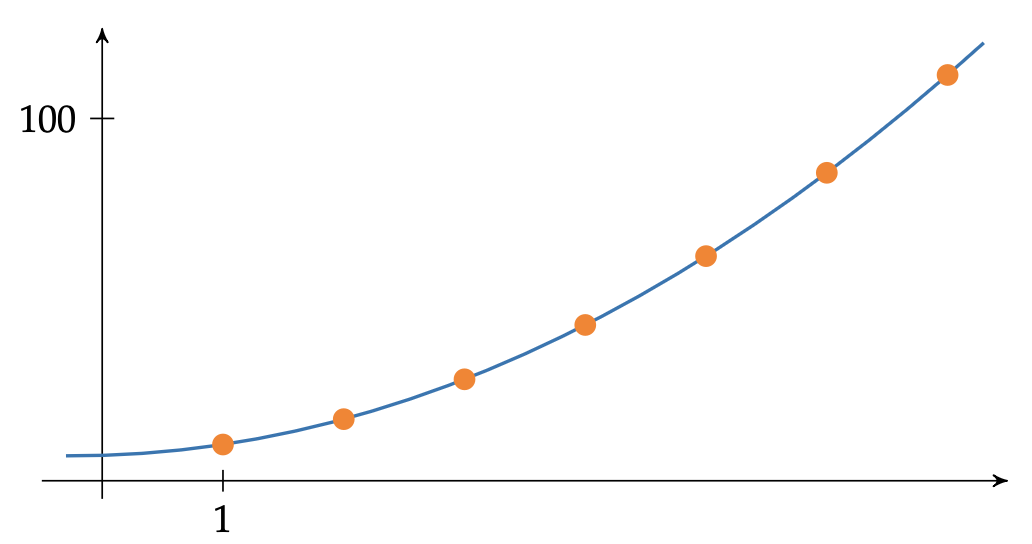
\includegraphics[width=\linewidth]{resources/images/RC_Parabel.png}
            \caption{Originale Kurve und Stützstellen}
            \label{fig:rs_original}
        \end{minipage}
        \hfill
        \begin{minipage}{0.48\textwidth}
            \centering
            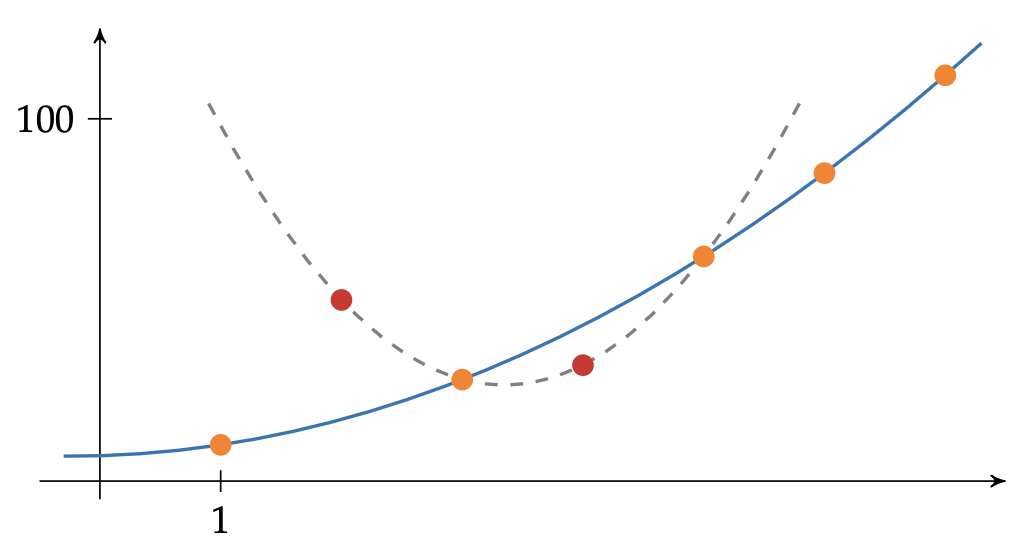
\includegraphics[width=\linewidth]{resources/images/RC_Fehlerparabel.png}
            \caption{Kurve mit fehlerhafter Stützstelle}
            \label{fig:rs_fehler}
        \end{minipage}
\end{figure}

Durch die Mehrheit der wahren Stützstellen gegenüber der fehlerhaften Stützstelle kann die ursprüngliche Kurve rekonstruiert werden. Dies ermöglicht es, die fehlerhaften Werte zu identifizieren und zu korrigieren. In diesem Beispiel können nicht mehr als zwei der richtigen Stützstellen auf der falschen Parabel liegen, dadurch ist die richtige Kurve eindeutig bestimmt. Dementsprechend ist die genaue Implementierung des Verfahrens davon abhängig, welche Arten von Fehlern erkannt und korrigiert werden sollen. Mit dem vorgestellten Beispiel ist es möglich, durch das Senden der sieben Funktionswerte \((10, 17, 28, 43, 62, 85, 112)\), die drei Zahlen \(2, 1, 7\) sicher zu übertragen. Bei unterschiedlichen Nachrichten unterscheiden sich die gesendeten Funktionswerte, aber nicht die Argumente die in der Prüfung und Berechnung verwendet werden. Die sichere Übertragung von Nachrichten aus drei Zahlen, beziehungsweise Symbolen, ist somit gewährleistet \cite{Springer_RS}.

Allgemein lässt sich dieses Verfahren wie folgt zusammenfassen: Eine Übertragung von \(k\) Symbolen, als Zahlen kodiert, nutzt eine Interpretation dieser Symbole als Polynom vom Grad \(k-1\). Der Sender sendet, um \(t\) Übertragungsfehler erfolgreich abzufangen, \(k + 2t\) Funktionswerte des Polynoms mit fest definierten Argumenten. Somit ist eine entsprechend sichere Übertragung garantiert \cite{Springer_RS}.

Um dieses Verfahren zu implementieren, muss wie beschrieben eine Polynominterpolation durchgeführt werden, um aus den Funktionswerten die ursprüngliche Nachricht zu rekonstruieren. Für eine realistische Implementierung ist eine Einschränkung nötig. Es werden in der Praxis ausschließlich endliche Körper verwendet. Dadurch ist außerdem die Anzahl der benötigten Bits für die Kodierung klar definiert. Jeder endliche Körper \(\mathbb{Z}_n\) weist mindestens eine primitive Einheitswurzel \(\alpha\) auf, für die folgendes gilt:

\begin{equation}
    \alpha^k \bmod n, \quad \text{mit } \mathbb{Z}_n \text{ und } k \in [1, n]
\end{equation}

\todo[inline]{Primitive Einheitswurzel erklären?}





%======================================
% 4. Fazit und Ausblick
%======================================
%!TEX root = ../main.tex

\chapter{Fazit und Ausblick}
\label{chap:fazit}



% \chapter{Beispiele}
% Beispiele, können problemlos entfernt werden!
% \section{Literatur}
% Beispiel Text \cite[S. 10]{testBuch1}
% Beispiel Homepage\cite{urlId} \\

% \section{Bilder}
% \begin{figure}[H]
% 	\centering
% 	
\includegraphics[width=0.3\linewidth]{resources/images/logo-dhbw}
% 	\caption{DHBW Logo}
% 	\label{fig:logo-dhbw}
% \end{figure}

% \section{Fußnote und Abkürzung}
% Fußnote\footnote{Fußnote}, \ac{DHBW}

% \section{Tabelle}
% \begin{table}[H]
% 	\centering
% 	\caption{Tabellenbeispiel}
% 	\label{tab:example}
% 	\begin{tabular}{|l|c|r|}
% 		\hline
% 		Spalte 1 & Spalte 2 & Spalte 3 \\
% 		\hline
% 		Zeile  &  &  \\
% 		\hline
% 		& Zeile &  \\
% 		\hline
% 		&  & Zeile \\
% 		\hline
% 		\multicolumn{2}{|r|}{Verbunden}	& nicht Verbunden \\
% 		\hline
% 	\end{tabular}
% \end{table}

% \underline{\section{Skript}
% \lstinline[language=c]|printf("Inline Code");|
% \lstinputlisting[language=python,caption={Beispiel python Skript},captionpos=t,label=scr:exanple]{resources/example-script.py}}

% \section{TODOs}
% Text Text\todo{TODO als Randnotiz} Text
% \todo[inline]{TODO als in Zeile}

% \begin{landscape}
% 	\section{Querformat}
% 	Text über Tabelle \ref{tab:breitetabelle}.
% 	\begin{table}[H]
% 		\caption{Breites Tabellenbeispiel}
% 		\label{tab:breitetabelle}
% 		\centering
% 		\resizebox{\columnwidth}{!}{%
% 			\begin{tabular}{|p{10cm}|p{10cm}|p{10cm}|}
% 				\hline
% 				Sehr & breite & Tabelle \\
% 				\hline
% 				\multicolumn{3}{|c|}{Tabelle wurde in der Größe verkleinert} \\
% 				\hline
% 			\end{tabular}
% 		}
% 	\end{table}
% 	Text unter Tabelle \ref{tab:breitetabelle}.
% \end{landscape}

% \section{Auflistungen}
% \begin{enumerate}
% 	\item Aufzählung nummeriert
% \end{enumerate}
% \begin{itemize}
% 	\item Aufzählung Stichpunkte
% \end{itemize}
% \begin{description}[style=nextline]
% 	\item[Label] Aufzählung als Beschreibung
% \end{description}
